\documentclass{report}
\usepackage[utf8]{inputenc}
\usepackage[spanish]{babel}
\usepackage[margin=2cm]{geometry}
\usepackage{graphicx}
\usepackage{float}
\usepackage{titlesec}
\usepackage{caption}
\usepackage{listings}
\usepackage{xcolor}
\usepackage{array}
\usepackage{booktabs}
\usepackage{tabularx}
\usepackage{multirow}
\usepackage{amsmath}
\usepackage{hyperref}
\usepackage{ragged2e} 
\usepackage{lipsum}

\definecolor{codegreen}{rgb}{0,0.6,0}
\definecolor{codegray}{rgb}{0.5,0.5,0.5}
\definecolor{codepurple}{rgb}{0.58,0,0.82}
\definecolor{backcolor}{rgb}{0.95,0.95,0.95}

\lstset{
    basicstyle=\ttfamily,
    inputencoding=utf8,
    extendedchars=true,
    literate=%
    {á}{{\'a}}1
    {é}{{\'e}}1
    {í}{{\'i}}1
    {ó}{{\'o}}1
    {ú}{{\'u}}1
    {ñ}{{\~n}}1
    {Á}{{\'A}}1
    {É}{{\'E}}1
    {Í}{{\'I}}1
    {Ó}{{\'O}}1
    {Ú}{{\'U}}1
    {Ñ}{{\~N}}1
}

\lstdefinestyle{mystyle}{
    backgroundcolor=\color{backcolor},
    commentstyle=\color{codegreen},
    keywordstyle=\color{red},
    numberstyle=\tiny\color{codegray},
    stringstyle=\color{codepurple},
    basicstyle=\ttfamily\footnotesize,
    breakatwhitespace=false,
    breaklines=true,
    captionpos=b,
    keepspaces=true,
    numbers=left,
    showspaces=false,
    showstringspaces=false,
    showtabs=false,
    tabsize=2  
}

\titleformat{\section}
{\huge\bfseries}{\thesection.}{1em}{}
\titleformat{\subsection}
{\large\bfseries}{\thesubsection}{1em}{}

\renewcommand\thesection{\arabic{section}}

\title{\Huge{\textbf{Diseño del Sistema}}\\
\Large{\textbf{Ingeniería de Software Para Sistemas Intelgentes}}}
\author{Diego Castillo Reyes\\Marthon Leobardo Yañez Martinez\\Aldo Escamilla Resendiz}

\graphicspath{{imagenes/}}

\begin{document}
\maketitle
\newpage

\section{Arquitectura del Sistema}
Para el diseño de la arquitectura del sistema se ha decidido utilizar una arquitectura orientada a servicios, es un enfoque que 
permite que los diferentes componentes de un sistema sean diseñados y desarrollados como servicios independientes que pueden 
interactuar entre sí. Esta arquitectura es útil cuando se busca crear un sistema modular, escalable y flexible, como en el caso 
del proyecto Thot, donde la interacción entre usuarios y el sistema depende de varios procesos interconectados 
(escaneo de QR, generación de trivias, eliminación de datos, etc.).

Los puntos clave para elegir esta arquitectura son:
\begin{itemize}
    \item \textbf{Escalabilidad:} Si en el futuro se quiere agregar nuevas salas al proyecto, simplemente se necesitaría crear nuevos servicios o extender 
    los existentes sin reestructurar todo el sistema. Por ejemplo, agregar una nueva sala solo requeriría añadir un nuevo conjunto de trivias o datos escaneables.
    \item \textbf{Mantenimiento Simplificado:} Como cada servicio es independiente, la detección y corrección de errores se limita al servicio afectado. Esto es 
    especialmente importante cuando se trabaja con distintos procesos como el manejo de usuarios y la generación de recompensas.
    \item \textbf{Flexibilidad:} SOA permite que diferentes equipos trabajen en servicios individuales de forma paralela, lo que 
    facilita el desarrollo colaborativo. Además, cada servicio puede escalarse de manera independiente, lo que es útil 
    si uno de ellos, como la generación de trivias, recibe más carga que otros.
\end{itemize}

Ahora bien, la arquitectura de Thot se compone de los siguientes servicios:
\begin{itemize}
    \item \textbf{Servicio de Autenticación de Usuarios:} Este servicio se encargaría de autenticar al usuario cuando escanea el primer código QR
    \begin{itemize}
        \item \textbf{Funcionalidad:} Registrar la edad del usuario para ajustar las trivias y generar la experiencia personalizada.
        \item \textbf{Interacción:} Envía la edad del usuario a los otros servicios para personalizar el contenido.
    \end{itemize}
    \item \textbf{Servicio de Escaneo de Códigos QR:} Gestiona la captura y el procesamiento de la información cuando un usuario escanea un código QR en la sala Mexica.
    \begin{itemize}
        \item \textbf{Funcionalidad:} Almacena temporalmente la información escaneada y la envía al servicio de generación de trivias.
        \item \textbf{Interacción:} Envía la información recopilada a los servicios de generación de trivias para crear una experiencia personalizada.
    \end{itemize}
    \item \textbf{Servicio de Almacenamiento Temporal de Datos:} Este servicio administra el almacenamiento temporal de los datos que el usuario genera durante su recorrido en la sala (información escaneada, progreso en la trivia, etc.).
    \begin{itemize}
        \item \textbf{Funcionalidad:} Guarda la información escaneada y la experiencia del usuario hasta que éste termine la visita. Elimina los datos cuando el usuario finaliza el recorrido.
        \item \textbf{Interacción:} Proporciona la información almacenada a los servicios de generación de trivias, y la envía al servicio de eliminación de datos al final.
    \end{itemize}
    \item \textbf{Servicio de Generación de Trivias:} Este servicio se encarga de generar las preguntas de la trivia basándose en la información que el usuario ha escaneado, adaptando el contenido según la edad y los intereses del usuario.
    \begin{itemize}
        \item \textbf{Funcionalidad:} Crear trivias personalizadas, asegurando que las preguntas se ajusten a la edad y los objetos de interés del usuario.
        \item \textbf{Interacción:} Recibe la información de los códigos QR escaneados y la edad del usuario del servicio de escaneo y almacenamiento de datos. Envia los resultados al servicio de recompensas.
    \end{itemize}
    \item \textbf{Servicio de Evaluación de Trivias:} Este servicio evalúa las respuestas del usuario en la trivia y calcula el puntaje.
    \begin{itemize}
        \item \textbf{Funcionalidad:} Calificar las respuestas del usuario y calcular el puntaje final.
        \item \textbf{Interacción:} Envía los resultados al servicio de eliminación de datos si el usuario finaliza su recorrido.
    \end{itemize}
    \item \textbf{Servicio de Eliminación Segura de Datos:} Se encarga de eliminar de manera segura la información temporal del usuario al finalizar su visita.
    \begin{itemize}
        \item \textbf{Funcionalidad:} Elimina todos los datos almacenados una vez que el usuario escanea el último QR de salida, cumpliendo con el requerimiento de no almacenar información personal.
        \item \textbf{Interacción:} Recibe la señal para eliminar los datos del servicio de escaneo de códigos QR o de evaluación de trivias, según cuando el usuario finalice su recorrido.
    \end{itemize}
    \item \textbf{Servicio de Administración de Contenidos:} Administra el contenido estático que alimenta al sistema (descripciones de objetos, preguntas de trivia, opciones de recompensas).
    \begin{itemize}
        \item \textbf{Funcionalidad:} Mantener y actualizar el contenido de la trivia y las descripciones que serán asociadas a los códigos QR.
        \item \textbf{Interacción:} Proporciona la información a los servicios de generación de trivias, asegurando que el contenido esté siempre actualizado.
    \end{itemize}
\end{itemize}

A continuación se explicará el flujo de interacción entre los servicios de Thot:
\begin{itemize}
    \item El usuario entra a la sala y escanea el primer código QR.
    \item El servicio de escaneo de QR procesa la información y la envía al servicio de almacenamiento temporal.
    \item A medida que el usuario escanea más códigos QR, la información se sigue almacenando.
    \item El usuario inicia una trivia. El servicio de generación de trivias crea las preguntas basadas en la información escaneada y la edad del usuario.
    \item El usuario responde la trivia, y el servicio de evaluación de trivias calcula el puntaje final.
    \item Si el puntaje es alto, el servicio de generación de recompensas crea una imagen personalizada para el usuario.
    \item Al final del recorrido, cuando el usuario escanea el último QR, el servicio de eliminación de datos borra toda la información temporal.
\end{itemize}

Finalmente se presenta el diagrama de secuencia de Thot:
\begin{figure}[H]
    \centering
    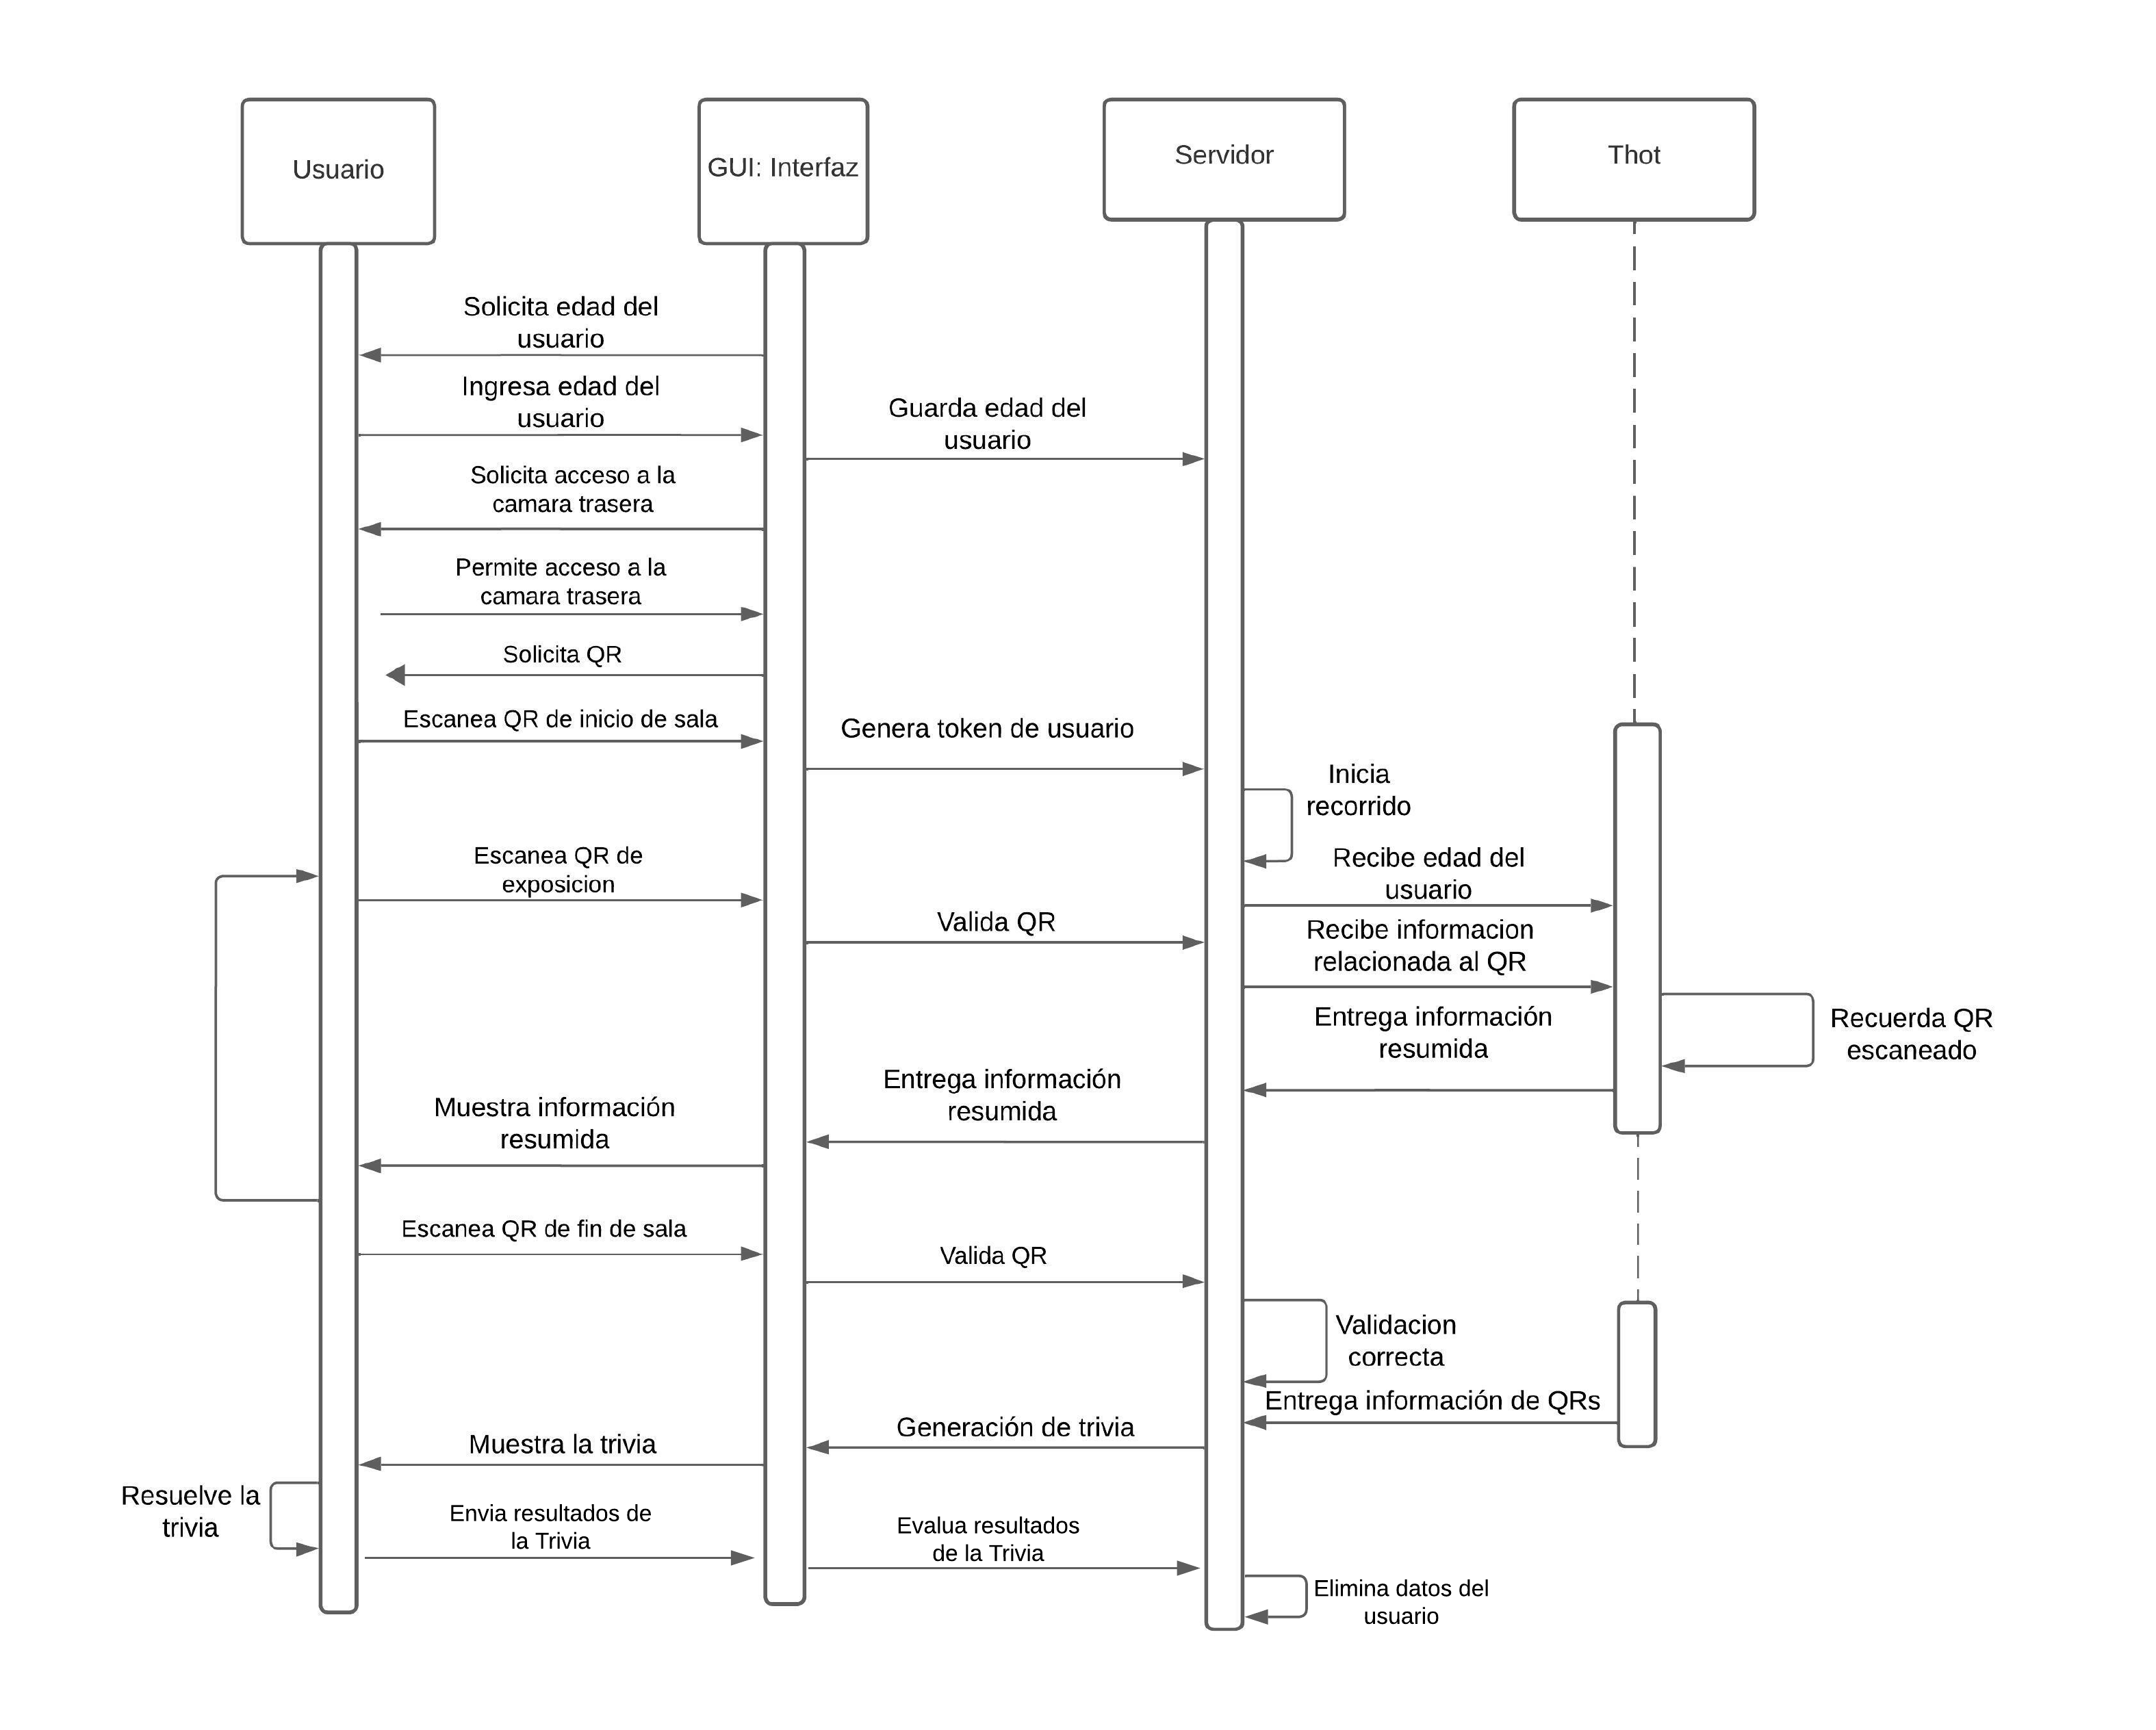
\includegraphics[width=0.8\textwidth]{DiagramaSecuenciaExp.png}
    \caption{Diagrama de Secuencia de la Interacción entre los Servicios de Thot}
\end{figure}
\section{Diseño de la Interfaz de Usuario}
\subsection{Diseño para Smartphones}
% agrega figuras para smartphones
\begin{figure}[H]
    \centering
    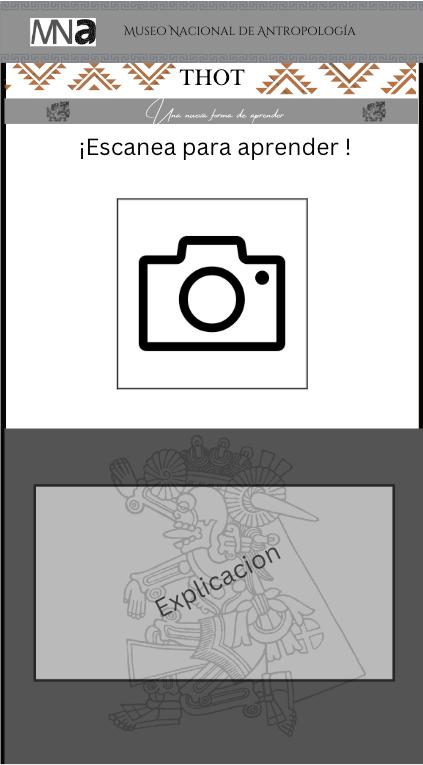
\includegraphics[width=0.8\textwidth]{interfazSP.jpeg}
    \caption{Diseño de la Interfaz de Usuario para Smartphones}
\end{figure}
\subsection{Diseño para Tablets}
% agrega figuras para tablets
\begin{figure}[H]
    \centering
    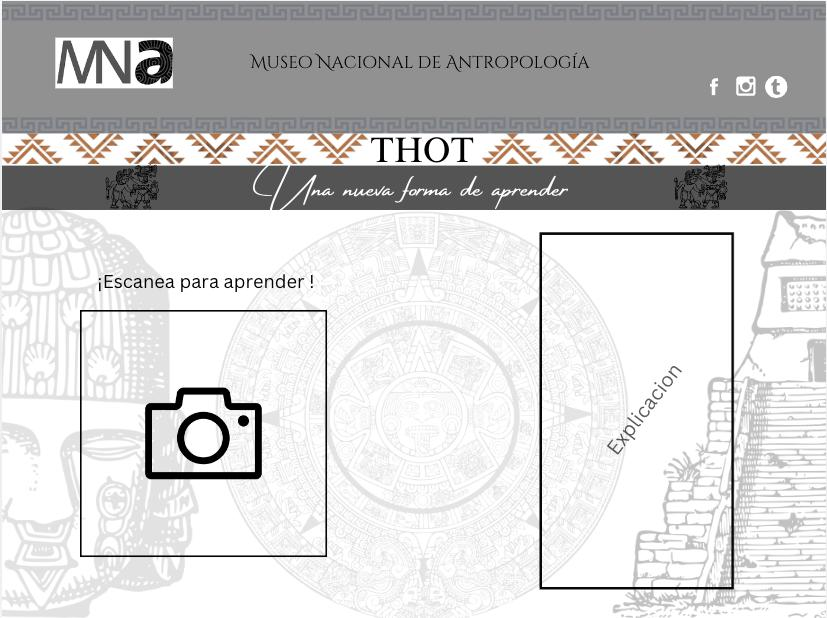
\includegraphics[width=0.8\textwidth]{interfazTablets.jpeg}
    \caption{Diseño de la Interfaz de Usuario para Tablets}
\end{figure}


\end{document}